\documentclass[10pt, conference, letterpaper]{IEEEtran}
\usepackage{cite}
\usepackage{xcolor,soul,framed}
\usepackage{amsmath,amssymb,amsfonts}
\usepackage{algorithmic}
\usepackage{graphicx}
\graphicspath{ {./images/} }

\begin{document}

    %=============================== TITLE ===============================%
    \title{
        Delay Optimal Dispatching with Observed Broadcast Replay in Two-Time Scale MDP
    }
    \author{
        \IEEEauthorblockN{HONG Yuncong}
        \IEEEauthorblockA{
            \textit{Department of CS}, The University of Hong Kong, China \\
            ychong@cs.hku.hk
        }
    }
    \maketitle

    %============================== ABSTRACT ==============================%
    \begin{abstract}
        \label{sec:abstract}
        We formulate the problem with job dispatching in distributed Edge Computing system, and we identify the difficulty exists in delayed cooperation between different APs (Access Points) and ESs (Edge Servers) to 
        \\
        (in progress)
    \end{abstract}

    \begin{IEEEkeywords}
        Edge Computing, Delayed Information, Two-time Scale MDP
    \end{IEEEkeywords}

    %============================ INTRODUCTION ============================%
    \begin{section}{INTRODUCTION}
        \label{sec:introduction}
        (in progress)
        \cite{sutton1998introduction}
    \end{section}

    %========================= LITERATURE REVIEW ==========================%
    % \begin{section}{LITERATURE REVIEW}
    %     \label{sec:review}
    % \end{section}

    %============================ FORMULATION =============================%
    \begin{section}{FORMULATION}
        \label{sec:formulation}
        In this section, we will firstly explain the problem definition about jobs dispatching in the edge computing system. Then we formulate this problem under a global MDP framework, which assumes a centralized agent could apply actions globally with updated states from each node. At last, we the global optimization problem into local optimization on each AP's side. We identify that by observing the collection of obsolete broadcast information under reasonable design, the problem turns out to be a two-time-scale MDP problem.

        \begin{subsection}{Problem Definition}
            In a Mobile Edge Computing system (MEC), the mobile users would firstly release their jobs to APs (Access Points), and APs make decision on which ES (Edge Servers) could better serve the job and dispatch them to corresponding ESs.
            In our problem, we identify the process of jobs from release to be processed. We call the length of lifetime as \emph{response time} and mainly composed of: waiting time on AP to make decision, uploading time from AP to ES, and total computation time on ES.
            
            The details about the communication model and computation model for jobs will be elaborated in the following subsection. And after that we will have one optimization definition for the general control problem with respect to dispatching and scheduling (but without constraints specified now).

            \begin{subsubsection}{Communication Model}
                The communication model in our system ignores the underlaid physical property and MAC design. We focus on the communication process of uploading of jobs.
                The assumed uploading time is deterministic and known in advance when the job is released to AP. The uploading time for one job may variance with respect to different ESs from the arrived AP, and the distribution of variance is not known in advance but is guaranteed with an expectation.
                Moreover, we assume the uploading process could be parallel among jobs, which implies infinite capacity. The infinite capacity could become reasonable with special design by discouraging jobs release from users with signaling, and thus make the capacity available is always finite.
                \\
                As we are going to apply dispatching action for jobs on AP side, all the AP and ES nodes need to broadcast for cooperation. The broadcast delay is considered deterministic and rather fixed {for simplified formulation}.
                The details of broadcast design about interval and contents will be elaborated in the \textit{Global Optimization Problem} section.
                For now, we don't take the broadcast cost into consideration because it's not been easily evaluated in the complicated network model (without specified).
            \end{subsubsection}

            \begin{subsubsection}{Computation Model}
                We assume that there is only one job being computed at one time on the edge server. The computation model is assumed to be deterministic, because the jobs to be computed on ESs are all considered released inside our system from Mobile Users.
                Moreover, we assume unrelated parallel machine model which implies that the computation time for one job is known when released but has no relationship with respect to any servers.
            \end{subsubsection}
            
            \begin{subsubsection}{Optimization Problem}
                We assume that there are $\mathcal{K}$ APs and $\mathcal{N}$ ESs in the MEC system.
                The arrival process of jobs at $k$-th AP is: $A^{(k)}(t)=I(t; (L_U, L_C))$ which is a indicator random process. It will return $0$ if no jobs arrive at $t$-th time slot, and return the job with property $(L_U, L_C)$ if one job arrives. $L_U, L_C$ are both vectors of length $\mathcal{N}$ denoting the deterministic uploading time and computation time respectively.
                $L_U$ is bounded by $T_U$ and $L_C$ is bounded by $T_C$, i.e. $L_U \in [1,T_U]$ and $L_C \in [1,T_C]$.
                \\
                For one job $j$, it will wait until the uploading decision is made for it; then it takes $L_U(n)$ time to be uploaded to $n$-th server; after uploaded, it will wait for its turn for computing until all the $L_C(n)$ components are processed and leave the system.
                \\
                Our optimization target is to minimize the average waiting time and computation time for each job, which is called the jobs' average response time. According to \emph{Little’s Law}, to minimize average response time, is equal to minimize the average number of jobs in a system, which is:
                \begin{gather}
                    \min_{\pi} \lim_{T \to \infty} E[\frac{1}{T} \sum_{t=0}^{T} N(t)]
                    \\
                    N(t) = \sum_{k \in \mathcal{K}} (A^{(k)}(t) + N_k(t))
                            + \sum_{n \in \mathcal{N}} N_n(t)
                \end{gather}
                where $N_k(t)$ denotes the number of jobs on $k$-th AP, and $N_n(t)$ denotes the number of jobs on $n$-th ES.
                The goal to minimize the cost caused by ESs could be simply achieved with heuristic algorithm \emph{SJF} (shortest-job first), because it is the fastest way to reduce number of jobs on the edge server. So, in the next MDP problems we will focus on the policy applied on AP side, and leave ES with fixed heuristic algorithm.
            \end{subsubsection}
        \end{subsection}

        \begin{subsection}{Global MDP Problem}
            In this section, we give out the formulation of the optimization problem under the framework of MDP. In this section, we firstly ignore the obsolete information brought by the broadcast delay and assume a centralized agent could observe the global states in real-time. This formulation could help better understanding the structure of the problem and analyzing the optimality gap from the real localized optimization elaborated in next section.

            \begin{subsubsection}{Markovian States}
                We adapt the description at grains of jobs and formulate the states into job sets at APs and ESs:
                \begin{gather*}
                    \mathbf{S}_g(t) \triangleq
                    \begin{Bmatrix}
                        S_{k}^{(W)}(t) = \{ (L_U, L_C) \}_{N_{k}^{(W)}}
                        \\
                        S_{k,n}^{(U)}(t)= \{ (L_C), L_{cd}^{(U)}(t) \}_{N_{k,n}^{(U)}}
                        \\
                        S_{n}^{(C)}(t)  = \{ L_{cd}^{(C)}(t) \}_{N_{n}^{(C)}}
                    \end{Bmatrix}
                    _{k \in [1,\mathcal{K}], n \in [1,\mathcal{N}]}
                \end{gather*}
                where $L_U, L_C$ are constant vectors of length $\mathcal{N}$, each denoting the uploading time and computation time of that job on each server; and $L^{(U)}_{cd}(t), L^{(C)}_{cd}(t)$ are countdowns for uploading and computing time remained for that job.
            \end{subsubsection}

            \begin{subsubsection}{Update Rules and Transition Function}
                \begin{figure}[h]
                    \centering
                    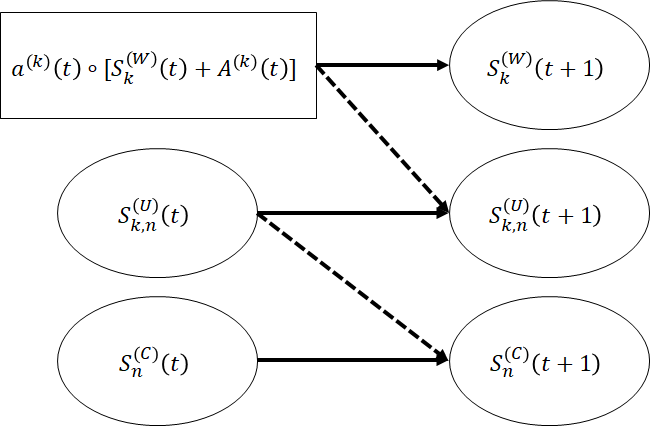
\includegraphics[width=0.45\textwidth]{single-transition.png}
                    \caption{Single-step transition function composing illustration}
                    \label{fig:trans}
                \end{figure}

                Firstly, we come up with some useful denotations for transmission expressed in figure \ref{fig:trans} as:
                \begin{align*}
                    I^{(W \to U)}_{k,n}(N;L) &\triangleq \{ (L_i),L^{(U)}_{cd}:=T^{br}_{k,n} \}_{i \in N}
                        \\
                    I^{(U \to C)}_{n}(N;L) &\triangleq \{ L^{(C)}_{cd}:=L_i \}_{i \in N}
                \end{align*}
                and we have the disturbance existing in the system as:
                \begin{gather*}
                    Pr\{ I^{(W \to U)}(t) | S_{k}^{(W)}(t),A^{(k)}(t), a(t) \}
                    \\
                        = Pr\{ A^{(k)}(t) \} \times \pi(a, \mathbf{S}'(t)|A^{(k)}(t))
                \end{gather*}
                where $I^{(W \to U)}(t)$ implies $S^{(W)}_{k}(t+1)$ and $S^{(U)}_{k,n}(t+1)$;

                The states transition on ES is easily obtained as following because the computation process on ES is deterministic:
                \begin{gather}
                    Pr\{ S_{n}^{(C)}(t+1) |S_{n}^{(C)}(t), (S_{k}^{(U)}(t))_{k \in [1,\mathcal{K}]} \} = 1
                \end{gather}
                The other interesting properties exists in the situation that when only states of ES is presence and the constraints are inversely put on APs. With \emph{Bayes' Law}, we could have:
                \begin{align}
                    & Pr\{ \sum{S_k(t)} | S_n(t,t+1) \} \nonumber\\
                    =& \frac{ Pr\{\sum{S_k(t)}\} \cdot Pr\{S_n(t,t+1)|\sum{S_k(t)}\} }{ Pr\{S_n(t,t+1)\} } \nonumber\\
                    =& \frac{
                            \prod_k Pr\{S_k(t)\}
                        }{
                            Pr\{S_n(t,t+1)\}
                        }
                \end{align}
                where $S_n(t,t+1) \triangleq S_{n}^{(C)}(t+1) |S_{n}^{(C)}(t)$, and $\sum{S_k(t)} \triangleq \{S_{k}^{(U)}(t)\}_{k \in [1,K]}$.
            \end{subsubsection}

            \begin{subsubsection}{Cost Function and Bellman Equation}
                According to the optimization target, we have the cost-to-go expression as followed:
                $$
                c(t) = \sum_{k \in \mathcal{K}}{|S^{(W)}_{k}(t)|}
                        + \sum_{k \in \mathcal{K}}\sum_{k \in \mathcal{N}}{|S^{(U)}_{k,n}(t)|}
                        + \sum_{k \in \mathcal{N}}{|S^{(C)}_{n}(t)|}
                $$
                The value equation in Bellman Equation format is as followed:
                $$
                V^{\pi}(S_g) = \sum_{S'_g} T(S_g, \pi(S_g), S'_g) (C(S_g') + \gamma V^{\pi}(S'_g))
                $$
                (need modification) where the dimension of possible $S'_g$ is:
                $$
                1 \times \sum{2^{|S^{(W)}_k|}} + (T_C \times T_U) \times \sum{2^{|S^{(W)}_k|+1}}
                $$
                and $C(S'_g)$ is the expectation of $c(t)$ given the arrival process as:
                \begin{align*}
                    C(S'_g) &= E[c(t)|(A^{(k)}(t))_{k \in [1,\mathcal{K}]}]
                    \\
                    &= 
                \end{align*}
            \end{subsubsection}
        \end{subsection}

        \begin{subsection}{Local MDP Problem}
            % TODO: stopped here
            As we are considering broadcast delay, we could re-consider the broadcast information as partially observed collected information lasting for $\hat{x}_k$ time slots.

            We formulate the local MDP optimization problem, with the same target as global value function. As the policy applied on each AP could not obtain the global information, we design the broadcast for every nodes to share their local states to other nodes (APs).
            
            However, due to the broadcast delay, we could not optimize the original global optimization problem based on states on one single AP. So we develop the local MDP problem with collected broadcast information.

            (given that broadcast delay is fixed, the length vector of fractions would be also fixed).

            \begin{subsubsection}{Broadcast Denotations}
                The illustration figure \ref{fig:brd} for single broadcast includes several important time points which are also important in multiple asynchronous broadcast: $x_{k,*}, d_{k,*}, T^{br}_{k,*}$
                \begin{figure}[h]
                    \centering
                    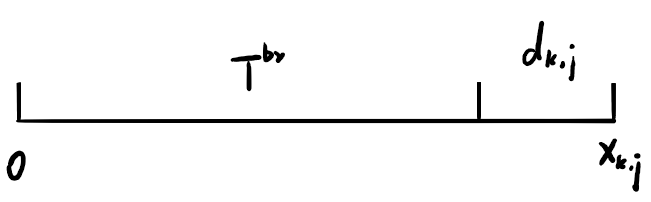
\includegraphics[width=0.45\textwidth]{single-broadcast.png}
                    \caption{Single broadcast timing illustration}
                    \label{fig:brd}
                \end{figure}
                And with the implication from the single broadcast, we generalize the conclusion for every broadcasts with:
                $$
                x_{k,*} = d_{k,*} + T^{Br}_{*}
                $$
                which takes a reasonable assumption that $T>d$ always ($*=k',n$ for $k$-th AP).

                Then we come up with the idea with collected broadcast states, which are split by the maximum broadcast interval which is denoted as $\hat{x}_k$:
                $$
                \hat{x}_k = \max(x_{k,*})
                $$
                And we denote all the partial or completed observed information (states of other nodes) in this smallest covering interval as $\Delta$.
                We notice that there is one periodic behavior as the broadcast interval is fixed for each node, and the period is simply obtained by LCM (Least Common Multiple):
                \begin{align*}
                    p_{k} &= \bar{x}_k/\hat{x}_k
                    \\
                    \bar{x}_k &= lcm(x_{k,*})
                \end{align*}
                And the series of states over time is denoted as:
                $$
                \{ \Delta^{(k)}_1 \to \dots \to \Delta^{(k)}_{p_k} \} \to \Delta_{1}
                $$
                
                The periodic behavior with the total $p_k$ behavior could be explained with \textit{information gap} in each period as $r_{k,*}$. Here we allows the time slot to be counted with $Z_+$, then we define the broadcast interval as \textit{additive modulo group} with respect to each node to $k$-th AP as $Z_{x_{k,*}}$. Then we find the gap in the periodic $\Delta_i$ is behaved in the remaining count-up way like:
                $$
                \hat{d}_{k,*}^{(i)} = i \times r_{k,*}
                $$
                where the remain is obtained by: $r_{k,*} \equiv \hat{x}_k \pmod{x_{k,*}}$.
            \end{subsubsection}

            \begin{subsubsection}{States Division in $\Delta_i$}
                We take the following series of states in the $k$-th AP local optimization problem, compared with global optimization problem with single-step MDP, we compose a non-aligned multi-step MDP with respect to asynchronous broadcast.
                \\
                The reason for taking states of length $p_k$ in stack is: this the shortest interval to online update the global information one-time; and in this form, we establish the model-based method for the optimization problem, but not considering learning model by predicting current cost/state. Although the information is updated, we have to endure the propagation delay with respect to relative larger broadcast interval (this information could take advantage with \emph{piggyback} the little partition of information during the broadcast)

                denote the *bounding time* of $S_*$ in $i$-th episode as: ($i \in [0, p_k]$):
                $$
                t^{(i)}_{k,*} = i \times \hat{x}_k - \hat{d}^{(i)}_{k,*}
                $$
                then we have all the states expression in $\Delta^{(k)}_i$-th period as:
                $$
                \{ S_*(t^{(i-1)}_{k,*}), S_*(t^{(i-1)}_{k,*}+1), \dots, S_*(t^{(i)}_{k,*}) \}_{* \in [1,k+n-1]}
                $$
                The states are denoted as previous mentioned:
                $$
                \Delta^{(k)}_{1}, \Delta^{(k)}_{2}, \dots, \Delta^{(k)}_{p_k}, \Delta^{(k)}_{1}, \Delta^{(k)}_{2}\dots
                $$
            \end{subsubsection}

            \begin{subsubsection}{Multi-step Update Rule}
                the multi-step transition is not simply iteratively run the single-step transition. Because the transition is confined by information from other nodes, the probability distribution would be deducted with Bayes' Law.

                Here we develope the rule for multi-step update.
                Action definition of the action generated in $\Delta_{i}$ as:
                $$
                a_{\vec{D_T}} = \{ a_{D_1}, \dots, a_{D_T} \}
                $$
                and the dimension is:
                $$
                \pi(a, \mathbf{\Delta}_i), |a_{\Delta_i}| \in \prod_{t \in \hat{x}_k} |2^{S^{(W)}(t)}|
                $$
                which is generated for all the possible states in next $\Delta_{i+1}$;

                Then we have some notations for short expression of the transition from $\Delta_{i}$ to $\Delta{i+1}$ as:
                \begin{align}
                    P_k(T,a) &\triangleq Pr\{ S^{(W,U)}_{k,D_T}|S^{(W,U)}_{k,D_1}, a_{\vec{D_T}},A^{(k)}_{\vec{D_T} }\}
                    \\
                    P_n(T) &\triangleq Pr\{ S^{(C)}_{n,D_T}|S^{(C)}_{n,D_1}, S^{(U)}_{k,\vec{D_T}} \}
                \end{align}
                and further more we have $\Delta \triangleq \{ \bar{P}_i, R_i, P_i \}$ where $R_i$ is consisted of states aligned at start and ending, $P_i$ is not aligned at ending, and $\bar{P}_i$ is not aligned at start and complement to $P_{i-1}$.

                The transition function of states $\Delta_i$ is composed of multiple single-step transitions, and impacted by inner deduction constraints due to Bayes' Law. We firstly give out the rules for update, and explain why the mathematical expression for transition function would be complex and not readable.
                \\
                (The update rule algorithm:)
                \begin{enumerate}
                    \item Complement Step: \\
                    Firstly given ES constraints to extend AP states and complete other ES states not given, until the bound without ES constraints, $\max(\hat{d}_{k,n}^{(i-1)})$;\\
                    Then given fixed AP to deduct AP and completes ES states until bound of $R_i$, $\max(\hat{d}^{(i-1)}_{k,*})$;
                    \item Aligned Expansion Step: \\
                    Simply carry out multi-step transition lasting for $( \hat{x}^{(i)}_k - \max(\hat{d}^{(i)}_{k,*}) )$
                    \item Non-aligned Expansion Step: \\
                    Firstly extends AP states to the maximum bound $\hat{x}^{(i)}_k$; \\
                    Then complements needed ES states with \emph{Total Probability Theorem} and remove the un-needed AP states (the removal process is safe for the given states are removed after sum-up of total probability)
                \end{enumerate}
                Therefore, we could not easily write out the transition probability without the length of each broadcast information specified.
            \end{subsubsection}

            \begin{subsubsection}{Total Transition and Bellman Equation}
                The total transition function could be obtained via the previous update rules, which we denote as $T(\Delta_{i-1}, a_{\Delta_{i-1}}, \Delta_{i})$
                \begin{itemize}
                    \item discounted factor for revised cost function
                    \item local cost function over $\Delta_i$
                \end{itemize}
            \end{subsubsection}

            \begin{subsubsection}{Optimality Gap to Global Optimization}
                (in progress)
                insight of optimality gap: action is fixed in the broadcast period;
            \end{subsubsection}
        \end{subsection}

    \end{section}

    %============================= ALGORITHM ==============================%
    \begin{section}{ALGORITHM}
        \label{sec:algorithm}
        (in progress)
    \end{section}

    %============================ EVALUATION ==============================%
    \begin{section}{EVALUATION}
        \label{sec:evaluation}
        (in progress)
    \end{section}

    %============================= CONCLUSION =============================%
    \begin{section}{CONCLUTION}
        \label{sec:conclusion}
        (in progress)
    \end{section}

    %============================== REFERENCE =============================%
    \bibliographystyle{IEEEtran}
    \bibliography{main.bib}
\end{document}